\chapter{Introduction} \label{chap:introduction}
Dies ist die Einleitung der schriftlichen Ausarbeitung.

\section{Abschnitte, Label und Referenzen} \label{sec:abschnitte}
Abschnitte werden mit dem Schlüsselwort $\backslash$section\{\} eingeleitet. Der Titel des Abschnitts steht dabei in geschweifen Klammern. Mit dem Befehl $\backslash$label\{\} können Marken im Text gesetzt werden, die mit dem Befehl $\backslash$ref\{\} referenziert werden. Der aktuelle Abschnitt befindet sich beispielsweise in Kap.~\ref{chap:introduction} und er hat die Nummer~\ref{sec:abschnitte}. Die Nummer wird automatisch erzeugt und auch ins Inhaltsverzeichnis geschrieben.

\subsection{Unterabschnitte}
gleiches Spiel jedoch mit $\backslash$subsection\{\}

Einige Zahlen mit Einheiten (hier wird automatisch ein Umbruch zwischen Zahl und Einheit verhindert):
\begin{itemize}
	\item Erdbeschleunigung: $g = \SI{9.81}{\meter\per\second\squared}$ oder auch $g = \SI{9.81}{m/s^{2}}$
    \item Lichtgeschwindigkeit: $c_0 = \SI{299792458}{\meter\per\second} = \SI{299792458}{m/s}$
\end{itemize}


\subsubsection{Noch eine Ebene tiefer...}
... kommt man mit $\backslash$subsubsection\{\}

\section{Abbildungen}
Hier einige Beispiele für Abbildungen.
\begin{figure}[htb]
	\centering
		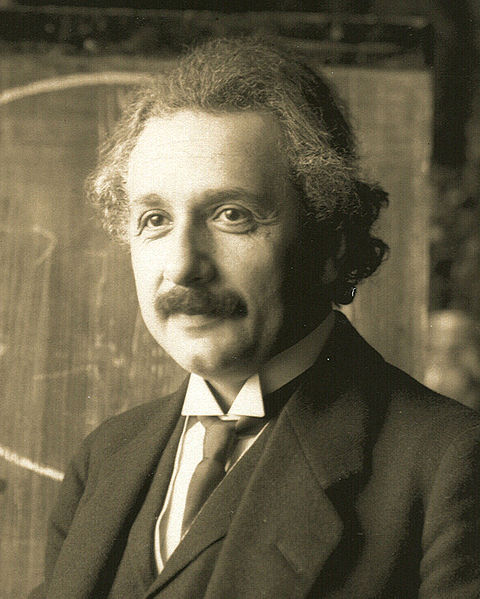
\includegraphics{Einstein}
	\caption{Ein großer Denker}
	\label{fig:Einstein}
\end{figure}


\begin{figure}[ht]
\centering
\subfloat[DER Denker schlechthin]{
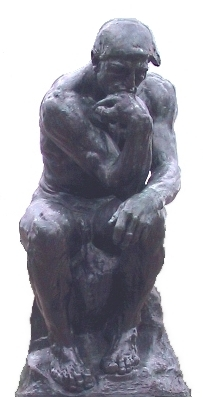
\includegraphics[width=0.275\textwidth]{Rodin-Denker-Kyoto}
\label{fig:subfig1}
} \qquad
\subfloat[noch ein Denker]{
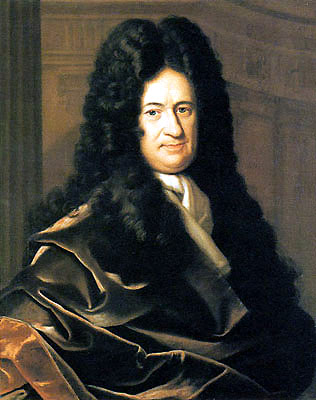
\includegraphics[width=0.4\textwidth]{Gottfried_Wilhelm_von_Leibniz}
\label{fig:subfig2}
}\\
\subfloat[und eine Denkerin]{
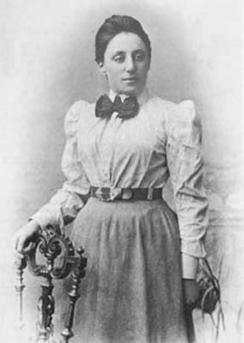
\includegraphics[width=0.4\textwidth]{Noether}
\label{fig:subfig3}
}
\caption[Kurzbeschreibung für Abbildungsindex]{Gemeinsame Beschriftung der drei Subfigures \subref{fig:subfig1}, \subref{fig:subfig2} and \subref{fig:subfig3}.
Hier auch mit längerem Text, um den Umbruch zu verdeutlichen.
Man sieht, dass der Abbildungstext links immer für sich steht.}
\label{fig:subfigureExample}
\end{figure}

\begin{figure}[ht]
\ContinuedFloat
\centering
\subfloat[DER Denker schlechthin]{
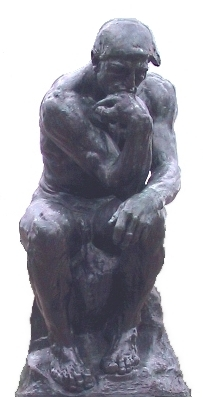
\includegraphics[width=0.275\textwidth]{Rodin-Denker-Kyoto}
\label{fig:subfig4}
} \qquad
\subfloat[noch ein Denker]{
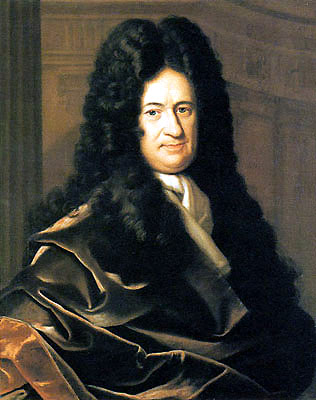
\includegraphics[width=0.4\textwidth]{Gottfried_Wilhelm_von_Leibniz}
\label{fig:subfig5}
}
\caption[Kurzbeschreibung für Abbildungsindex (Fortsetzung)]{Eine Fortsetzung der letzten Abbildung für viele Bilder.
Gemeinsame Beschriftung der zwei Subfigures \subref{fig:subfig4}, \subref{fig:subfig5}}
\label{fig:subfigureExampleCont}
\end{figure}